\section{\Multidispatch{} Linearizability}
\label{sec:mdl}

In this section, we define our new consistency model and show how
applications can be transformed for interaction with an \multidispatch{} Linearizeable system to reap performance benefits while appearing to behave identically to users. We conclude with a discussion and proof of our external equivalence result.

\todo{Make a pass to see if there is anything defined that we don't use and thus that we can cut.}


\subsection{Definition}
\label{sec:mdl:def}


To define \mdl{}, we first introduce necessary terminology. As described in ~\ref{sec:motivation}, application processes interact with a back-end \textit{system} (e.g., a database or key-value store),
which is defined by its \textit{operations} and a
\textit{specification}~\cite{herlihy1990linearizability,lynch1996da}. An
\textit{operation} comprises pairs of \textit{invocations}, specifying the
operation's arguments, and matching \textit{responses}, containing
return values. The \textit{specification} is a
% prefix-closed
set of sequences of
invocation-response pairs defining the system's correct behavior in the absence
of concurrency. A sequence $S$ in a specification $\spec$ defines a total order
over its operations, denoted $<_S$.

An application's processes, $P_i$, define a set of \textit{executions},
which are sequences of alternating \textit{states} and
\textit{actions}. The \textit{actions} we will focus on are the operations, $o_i$, issued to the back-end system.
% and the $i$th component of each state in $\alpha$.
We say an
operation is \textit{complete} if its invocation has a matching response in
$\alpha$. We denote $\complete(\alpha)$ as the maximal subsequence of $\alpha$
comprising only complete operations~\cite{herlihy1990linearizability}. 

Given an execution $\alpha$, we will often refer to an individual process's
\textit{sub-execution}, denoted $\alpha|P_i$. $\alpha|P_i$ comprises
only $P_i$'s actions. Given a sequence of complete actions,
$\complete(\alpha)$, we define $\complete(\alpha)||P$ as the
\textit{sequentialization} of $P$'s operations in $\complete(\alpha)$.
$\complete(\alpha)||P$ is found by, for each operation $o$, shifting $o$'s response
$\res(o)$ left in $\complete(\alpha)|P$ until it immediately follows $o$'s
invocation $\inv(o)$.
Importantly, this maintains a process's
\textit{issue order}, the order it invoked its operations. Intuitively, it translates the execution to a sequential one.
Finally, two operations in an execution $\alpha$ are
ordered in real time~\cite{herlihy1990linearizability}, denoted
$o_1 \rt_\alpha o_2$, if $\res(o_1)$ precedes $\inv(o_2)$ in $\alpha$.

We are now ready to define our new consistency model.
\paragraph{\Multidispatch{} Linearizability.} An execution $\alpha_1$ satisfies \textit{\multidispatch{} linearizability} if it
can be extended, by adding zero or more responses, to create $\alpha_2$ such that
there exists a sequence $S \in \spec$ where 
\begin{enumerate}
    \item for all $P$,
$S|P = \complete(\alpha_2)||P$
    \item for all pairs of operations
$o_1$ and $o_2$, \\$o_1 \rt_{\alpha_1} o_2 \implies o_1 <_S o_2$.
\end{enumerate}

In plain language, an \MDL{} system guarantees it reflects a total order 
over operations, just like traditional Linearizability. This order (1) guarantees to preserve each process's issue order and (2) guarantees the real-time order of operations, as in traditional Linearizability. The key difference is individual processes' concurrent operations appear to take effect in invocation order sequentially.

\wl{Need a consistency pass to use the same suffix-closed/complete failure \{semantics\} or not everywhere}

\ak{Some reviewers didn't like the idea that you can't "remove" these guarantees, ie they think it's necessary to have the option to have no ordering guarantees for concurrent ops when you don't want/need it (to bypass coordination overhead). Wondering if we should make it explicit that that's still very possible if a process spawns many new threads (and has distinct client IDs)? or if programmer uses some library that effectively abstracts that away? or what about the single-process cases where you can safely issue everything in parallel?}
%\subsubsection{Suffix-Closed Failures}
\paragraph{Suffix-Closed Failures.}
\label{sec:mdl:def:failures}

\MDL{}'s definition has an important implication for system designers.
In systems where operations can fail (even temporarily before being retried), the
effects of an operation cannot be exposed to other processes until all of its 
predecessors are guaranteed to succeed. Doing so would violate the intuitively
correct behavior of most systems, and formally, this would result in
$S|P \neq \complete(\alpha_2)||P$ for all legal sequential histories
$S \in \spec$.
We refer to this property as \textit{suffix-closed failure semantics}.
%\true{( example in \cref{subfig:suffix_closed_breaks} from the previous section, the return values r(n)=1, r(m)=0 violate this property because w(n=1) is observed by r(n)=1 and }


In an \MDL{} system, suffix-closed failures must be guaranteed even in the
face of concurrent operations from the same process, potentially to
objects on different shards. Drawing again on the example in figure ~\ref{fig:retwissequential}, if the operations from the yellow block are sent concurrently from the same process to an \mdl back-end and any of the operations from the loop on line 4 fail, then the remaining operations in the loop on line 4 and lines 6 and 7 must also fail regardless of whether any of them could succeed. \ak{this might be a bad example cuz now \textit{some} followers will see the object, but the poster won't and some other followers won't? really, line 5 should be atomic... and we could say if line 5 fails, then definitely lines 6 and 7 will.} As we will see in Section~\ref{sec:mdl:zookeeper},
guaranteeing suffix-closed failures is one way in which existing systems do not provide \mdl{}.  

\wl{Should we punch up this discussion? I think it's a major way we're different from A-Linearizability and its necessary! For instance, we need this for our equivalence result right?! That seems important!}

\subsection{Transforming Applications}
\label{sec:mdl:equivalence}

\begin{figure}

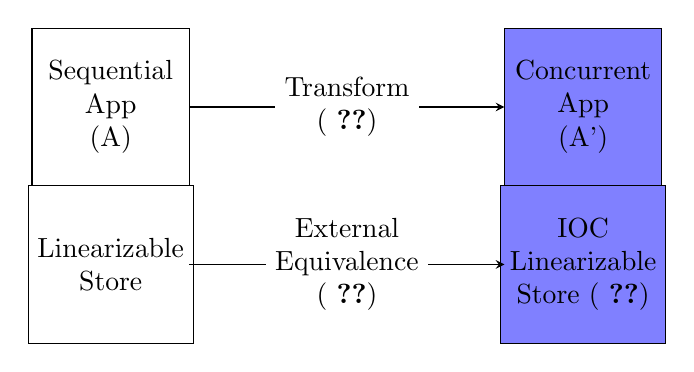
\begin{tikzpicture}
 
\node (appbox) [draw,
    minimum size=2cm,
    xshift=-3cm,
    align=center,
    yshift=2cm
] {Sequential\\App\\(A)};

\node (linstore) [draw,
    minimum size=2cm,
    align=center,
    xshift=-3cm
] {Linearizable\\Store};

\node (mdapp) [draw,
    minimum size=2cm,
    xshift=3cm,
    align=center,
    yshift=2cm,
    fill=blue!50
] {Concurrent\\App\\(A')};

\node (mdlinstore) [draw,
    minimum size=2cm,
    xshift=3cm,
    align=center,
    fill=blue!50
] {IOC\\Linearizable\\Store (~\ref{sec:mdl:def})};

% \draw [stealth-](1.5,2) --  node[midway,fill=white]{$coord$}(-1.5, 2);


\draw [stealth-](2,2) --  node[midway,fill=white,align=center]{Transform\\(~\ref{sec:mdl:equivalence})}(-2, 2);

\draw [stealth-](2,0) --  node[midway,fill=white, align=center]{External\\Equivalence\\(~\ref{sec:mdl:exteq})}(-2, 0);

\end{tikzpicture}
\centering
\caption{Architecture of usage}
\label{fig:transform}
\end{figure}

In this section, we show how we can transform a sequential application that interacts with
a traditional linearizable system into a concurrent application to take advantage of a \mdl{} system, as shown in ~\ref{fig:transform}. Importantly, our transformation will ensure that the new
application appears to behave identically to the original application (as far as
the users can tell), or, that the two applications are \textit{externally equivalent}, an equivalence result we then prove.

% We first define the transformation and several preliminaries. We then
% present a condensed form of the proof that the transformation preserves external
% equivalence. (A complete proof can be found in Appendix A.) %~\ref{sec:equivalence}.)
% For ease of exposition, we focus on the actions within an
% execution and assume states can be modified and reordered as needed.

%\subsubsection{Parallelizing Applications}
\paragraph{Making Sequential Applications Concurrent.}
\label{sec:mdl:transform}

We describe how to transform an application $A$ that is built to
interact with a linearizable system to produce a new application
$A^\prime = \transform(A)$ that can interact with a comparable \MDL{} system.
We attempt to describe this transformation in generic terms, independent of any particular programming language.

The first step is to replace synchronous, system-facing I/O with
futures. This allows operation invocations and responses
to be reordered in $A$ with respect to other actions (i.e., instructions).
The aim is to then move operation invocations earlier such that the application
can issue multiple operations concurrently and reap the performance benefits 
of an \MDL{} system.

To produce the new application $A^\prime$, we then move actions in $A$ before prior 
actions provided $A^\prime$ maintains the following:
\textbf{(R1)} the order of data-dependent actions within
each process of $A$,
\textbf{(R2)} the control flow of each process in $A$,
\textbf{(R3)} the issue order of $A$'s operations,
\textbf{(R4)} the order of non-system-facing external
actions in $A$, including messages to/from users,
\textbf{(R5)} the order between a non-system-facing external 
actions and operation invocations (in particular, the first invocation in a
sequence of operations), and
\textbf{(R6)} the order between non-system-facing external actions and operation responses (e.g., by waiting for the successful responses of any outstanding operations before sending a message to a user).

An example of the transform is shown in figure ~\ref{fig:retwis-post2}\subref{fig:retwistransform}. Mainly, all of the calls made to the back-end system have been replaced with futures, allowing each of them to be concurrent with one another, and synchronization points have been added to respect data-dependencies. It is also worth noting \mdl{} makes no guarantees on the response order of operations. On line 11, it suffices to wait on just \texttt{\$future3} to return because none of the preceding operations require a return value. It is unclear if the previous operations have returned at the time of \texttt{\$future3} returning a value, but because of suffix-closed failure and invocation ordering guarantees, it is guaranteed they will succeed and take effect before the operation associated with \texttt{\$future3} takes effect.

\subsection{External Equivalence}
\label{sec:mdl:exteq}
So far we have defined a new consistency model for back-end systems and we have shown how to transform applications interacting with these systems. Finally, we show that users cannot tell the difference between interacting with the transformed applications working atop back-end systems guaranteeing \mdl{} and the sequential versions of those applications that interact with Linearizable back-ends. More formally, we can state this result, which we call External Equivalence, as the following theorem:
% externally equivalent executions are indistinguishable to users.

\begin{thm}
Let $A$ be an application designed to interact with a linearizable system,
and let $A^\prime = \transform(A)$ be the transformed application. Suppose
$\alpha^\prime$ is an execution of $A^\prime$ that satisfies
\MDL{}. Then there is an externally equivalent execution $\beta$
of $A$ that satisfies linearizability.
\end{thm}

% \begin{proof}
The proof proceeds in steps: First, we create an execution $\alpha$ from
$\alpha^\prime$ by essentially undoing the parallelizing transformation in
each process's sub-execution. Second, we produce $\beta$ by fixing the order
of operations across processes to ensure $\beta$ is well-formed and satisfies linearizability. A complete proof of the result can be found in the appendix. 

% By the assumption that $A$ is well-formed and the rules of $\transform$,
% each $\alpha^\prime | P_i$ comprises sub-sequences of local and
% system-facing actions separated by non-system-facing external actions.
% Further, by \textbf{R4}, the order of the non-system-facing external
% actions in each $\alpha^\prime | P_i$ respects the program order of the
% original application $A$. 

% We first reorder the actions in each sub-sequence of each $\alpha^\prime | P_i$
% to place the local and system-facing actions such that they respect $A$'s program
% order. More precisely, for each $\alpha^\prime | P_i$, starting with the right-most
% action $\pi$, shift $\pi$ left in $\alpha^\prime$ until it precedes
% all other actions $\pi^\prime$ in $\alpha^\prime | P_i$ such that $A$'s program
% order requires it. Let $\alpha^\prime$ be the resulting execution.

% By the observation about each $\alpha^\prime | P_i$ above, the order of
% non-system-facing external actions in $\alpha$ respects $A$'s program order
% (because $A^\prime$'s is identical). Further, each $\alpha | P_i$ now
% issues its operations sequentially (since $A$'s program order requires it).
% Lastly, by \MDL{}'s suffix-closed failure semantics, all of a process's 
% completed operations precede any failed ones.

% The execution $\alpha$, however, may not satisfy linearizability. We remedy this
% and produce the needed $\beta$. To do so, first recall that by assumption the 
% original  $\alpha^\prime$ satisfies \MDL{}, so let $<_S$ (for $S \in \spec$) be the total order over the operations in $\alpha^\prime$, as guaranteed by \MDL{}.

% Let $\prec_{\alpha}$ be the transitive closure of following pairs of actions
% $(\pi_i, \pi_j)$ in $\alpha$:
% \begin{enumerate}
%     \item $\mathbf{\prec_{P_i}}$\textbf{:} $\pi_i$ precedes $\pi_j$ in some $\alpha | P_i$,
%     \item $\mathbf{\prec_U}$\textbf{:} $\pi_i$ precedes $\pi_j$ in $\alpha | U$, or
%     \item $\mathbf{\prec_S}$\textbf{:} For each adjacent pair $o_k$, $o_{k+1}$
%     in $S$, $\pi_i$ is $o_k$'s response and $\pi_j$ is $o_{k+1}$'s invocation.
% \end{enumerate}

% We posit $\prec_{\alpha}$ defines an irreflexive partial order
% over the actions in $\alpha$. Clearly it is irreflexive; we now prove
% it is acyclic and transitive.

% For sake of contradiction, assume $\prec_{\alpha}$ contains a cycle, and
% let $\pi_1 \prec_{\alpha} \pi_2 \prec_{\alpha} \ldots \prec_{\alpha} \pi_1$
% be a shortest cycle that does not include any transitive edges.

% We first prove several important properties of the cycle:
% \textbf{(P1)} The cycle contains at least two actions.
% This follows from the definitions of $\prec_{P_i}$,
% $\prec_U$, and $\prec_S$.
% \textbf{(P2)} The cycle does not contain two consecutive
% $\prec_{P_i}$ edges or two consecutive $\prec_U$ edges. Otherwise, a 
% shorter cycle exists since $\prec_{P_i}$ and $\prec_U$ are transitive.
% \textbf{(P3)} The cycle does not contain two consecutive $\prec_S$. This follows from the 
% definitions of $\prec_S$.

% In the remainder of the proof, we leverage the following lemma. 
% For sake of brevity, however, we omit its proof.

% \begin{lem}
%     Let $\pi_1 \prec_{\alpha} \ldots \prec_{\alpha} \pi_n$
%     be a sequence of $n$ actions connected any of
%     $\prec_{P_i}$, $\prec_U$, and $\prec_S$ edges, and further
%     assume $\pi_1$ and $\pi_n$ are send-to or receive-from actions.
%     Then $\pi_1$ precedes $\pi_n$ in $\alpha$.
%     \label{lem:helper2}
% \end{lem}

% We continue the proof by cases: First, assume the cycle contains at least one $\prec_U$ edge. Then the cycle can be
% written as
% $\pi_1 \prec_U \pi_2 \prec_{\alpha} \ldots \prec_{\alpha} \pi_n \prec_{\alpha} \pi_1$. By the definition of $<_U$, clearly $\pi_1$ precedes $\pi_2$ in $\alpha$.

% Since users interact with processes using channels, $\pi_2$ and
% $\pi_1$ are either receive-from or send-to actions,
% so the remainder of the cycle
% $\pi_2 \prec_{\alpha} \ldots \prec_{\alpha} \pi_1$
% is a sequence of actions connected by $\prec_{P_i}$, $\prec_U$, and $\prec_S$ edges
% starting and ending with a send-to or a receive-from action.
% Thus, by Lemma~\ref{lem:helper2}, $\pi_2$ precedes $\pi_1$ in $\alpha$,
% a contradiction.

% Second, assume the cycle does not contain any $\prec_U$ edges.
% By Properties \textbf{P2} and \textbf{P3}, the cycle comprises alternating
% $\prec_{P_i}$ and $\prec_S$ edges. Also, all $P_i$ in the $\prec_{P_i}$
% must be distinct, otherwise a shorter cycle must exist.
% Lastly, since they alternate with $\prec_S$ edges,
% for each $\pi_i \prec_{P_i} \pi_{i+1}$, we know 
% $\pi_i$ is an invocation and $\pi_{i+1}$ is a response.

% By definition of $\prec_{P_i}$, $\pi_i$ precedes $\pi_{i+1}$ in $\alpha | P_i$.
% Since each process’s system interactions occur sequentially in $\alpha$,
% $\pi_{i}$ must also precede $\pi_{i+1}$'s corresponding invocation.
% Since the transformation between $A$ and $A^\prime$ preserves each process’s
% invocation order (as does MDL), this implies $\op(\pi_{i})$ is ordered in $S$
% before $\op(\pi_{i+1})$.

% As a result, for each $\pi_i \prec_{P_i} \pi_{i+1}$ in our cycle, we can replace it
% with a sequence of $\prec_{P_i}$ and $\prec_S$ edges that includes the invocations 
% and responses of all operations in $S$ between $\op(\pi_i)$ and $\op(\pi_{i+1})$
% (if any). This (no longer shortest) cycle implies there is a cycle over operations 
% in $S$. But this contradicts the definition of $S$, which is a 
% total order. Thus, $\prec_{\alpha}$ is acyclic. Combined with the
% definitions of $\prec_{P_i}$, $\prec_U$, and $\prec_S$, this also
% shows it is irreflexive.

% Let $\beta$ be a topological sort of $\prec_{\alpha}$ on the actions in
% $\alpha$. To conclude the proof, we show $\beta$ is well-formed,
% satisfies linearizability, and is externally equivalent to $\alpha^\prime$.

% The fact that $\beta$ is well-formed follows from the definition of
% $\prec_{\alpha}$. It preserves the order of user-facing actions,
% which were unaltered in the transformation from $\alpha^\prime$ to $\alpha$.
% Similarly, it preserves the order of each message's send-to and receive-from actions,
% and their order was also unaltered in producing $\alpha$. Finally, the original
% transformation to $\alpha$ placed the actions of each $\alpha | P_i$ in
% the order dictated by $A$'s program order, and this was preserved by
% $\prec_{\alpha}$ in producing $\beta$.

% By the initial reordering to produce $\alpha$ and the definition of
% $\prec_{\alpha}$, the operations across all processes in $\beta$
% are sequential in the order defined by $S$. Since $<_S$ defines a
% total order over all operations, $\beta$ thus satisfies linearizability.

% Finally, since the initial transformation from $\alpha^\prime$ to $\alpha$
% did not alter the order of any user-facing actions, clearly
% $\alpha^\prime | U = \alpha | U$. Then by the definition of $\prec_{\alpha}$, 
% $\alpha | U = \beta | U$. $\beta$ is thus externally equivalent to $\alpha$.
% \end{proof}
